\RequirePackage{xcolor}
\documentclass[a4]{sciposter}
\usepackage{multicol,subfig,amsmath} % columnas, figuras, ecuaciones
\usepackage{graphicx,url,hyperref,doi}
\hypersetup{hidelinks}  
\usepackage[utf8]{inputenc}
\usepackage[sort&compress,numbers]{natbib}
\usepackage[font=small,labelfont=bf]{caption}

\usepackage{tikz} % diagramas
\tikzstyle{elem} = [draw, rectangle, thick, minimum height=2em, minimum width=2em]
\tikzstyle{line} = [draw, thick, -stealth, shorten >=1pt]
\usepackage{dingbat}

\setlength{\parskip}{3pt} % espacio entre parrafos
\renewcommand{\arraystretch}{1} % altura de renglones de cuadros

\title{Sentiment Analysis through Conversational Data}
\author{Alexander Espronceda Gómez}
\institute {Facultad de Ingeniería Mecánica y Eléctrica}
\email{alexander.esproncedago@uanl.edu.mx}

\leftlogo[1]{uanl.png} 
\rightlogo[1]{fime.png}

\begin{document}

\conference{Facultad de Ingeniería Mecánica y Eléctrica ---
  Universidad Autónoma de Nuevo León}

\maketitle
\begin{abstract}
In this thesis, open-sourced software is proposed, which interprets the text entered by a person and determines how they are feeling at the moment, with the purpose of being used in tandem with another software or algorithms focused on conversational data.
The study method used will make a comprehensive analysis of neural networks, as well as pattern recognition and data collection.
The algorithm is open-source so anyone can add or remove modules as needed.
\end{abstract}

\begin{multicols}{3} 

\section{Introduction}
Human beings are social beings, this is widely known. To survive, we must band together and communicate with each other, bonding in the process. This is thanks to a neural process called \textit{empathy}, which is defined as a process that happens in our brains.
\begin{figure}[!h]
	\centering
	\includegraphics[scale=0.2]{BrainMap}
	\label{fig:brainmap}
	\captionsetup{type=figure}
	\setcounter{figure}{0}
	\caption{Lateral brain map of the parts in charge of the empathy processes. Drawing generated using BrainPainter \citep{img1}.}
\end{figure}

Theoretically, a machine could be taught to process signals of distress and react accordingly using a machine learning algorithm.

\section{Justification}
This project could prove especially useful towards being used in projects designed for people who have trouble discerning when to console someone or having an idea of how other people or even themselves feel, such as the case of people with Asperger's Syndrome or other forms of high-functioning autism.
To this end, the decision was made to work on this project.

\section{Hypothesis}
The hypothesis of this thesis is that using supervised machine learning with a neural network could accurately classify the sentiment behind an input text as ``Good'', ``Neutral'' or ``Bad'', with the purpose of being implemented in tandem with another software or algorithms focused on conversational data.

\section{Objectives}
The objective of this project is to make software capable of determining how the person that writes the input text is feeling according to the words in it, while keeping the code open-source so it can be used in other projects. This could be achieved thanks to the technology present in machine learning algorithms and an extensive amount of datasets.

\section{Background}
\subsection{Basic Concepts}
\begin{description}
	\item[Machine Learning]{Also known as ML. The type of algorithm needed for automatic processing, making the machine ``learn'' (hence the name) over time given enough data.}
	\item[Neural Network]{A Machine Learning algorithm that uses weights and filters to output data.}
	\item[Natural Language Processing]{This is the method used for the algorithm to understand the content of the sentences, this is usually achieved by using tokenization but a preset corpus can also be used.}	
	\item[Sentiment Analysis]{This involves a ML algorithm, usually a Neural Network, that is able to analyze sentences and classify them according to the words used.}
	\item[Corpus]{Preset internal dictionary that the algorithm uses.}
	\item[Tokenizing]{Process that converts every word in the lexicon to an assigned number for easier processing}
\end{description}

\section{Comparison to Related Work}
There are several papers on similar projects, the following table marks the specifics of each one's relevant features compared to this project's.
\begin{table}[!h]
	\captionsetup{type=table}
	\setcounter{table}{0}
	\caption{Comparison between existing literature and the present work: \checkmark indicates the fulfillment of a criterion, otherwise $\times$ is used.}
	\vspace{0.5cm}
	\centering
	\begin{tabular}[t]{|l|l|l|l|l|l|}
	\hline
		\textbf{Project} & \rotatebox{90}{\textbf{Neural Network}} & \rotatebox{90}{\textbf{Text Processing}} & \rotatebox{90}{\textbf{Sentiment Analysis }} & \rotatebox{90}{\textbf{Open Source}} & \rotatebox{90}{\textbf{Modular}}
	\\ \hline
	\citet{rf10} Maximum Entropy & \checkmark & \checkmark & \checkmark & $\times$ & $\times$
	\\ \hline
	\citet{rf10} Support Vector Machines & \checkmark & \checkmark & \checkmark & $\times$ & $\times$
	\\ \hline
	\citet{rf10} Lingpipe & \checkmark & \checkmark & \checkmark &  $\times$ & $\times$
	\\ \hline
	\citet{rf6} & \checkmark & \checkmark & \checkmark &  $\times$ & $\times$
	\\ \hline
	\citet{rf14} & \checkmark & \checkmark & $\times$ & \checkmark & $\times$
	\\ \hline
	\citet{rf5} & \checkmark & \checkmark & \checkmark & \checkmark & $\times$
	\\ \hline
	\citet{rf11} & \checkmark & \checkmark & $\times$ &  \checkmark & $\times$
	\\ \hline
	\citet{rf12} & \checkmark & \checkmark & \checkmark &  \checkmark & $\times$
	\\ \hline
	\citet{rf13} & \checkmark & \checkmark & \checkmark & $\times$ & $\times$
	\\ \hline
	\citet{rf15} & \checkmark & \checkmark & $\times$ &  \checkmark & $\times$
	\\ \hline
	\citet{rf16} & \checkmark & \checkmark & \checkmark & \checkmark & $\times$
	\\ \hline
	The present work & \checkmark & \checkmark & \checkmark & \checkmark & \checkmark
	\\ \hline
	\end{tabular}
\end{table}

\section{Proposed Solution}
This project is built on Python v3.8.10, The libraries used for this project to come to fruition are TensorFlow v2.6.0 and Keras v2.6.0 for the Neural Network section and Natural Language Toolkit v3.5 (also known as NLTK) for the tokenization and stemming process.
\begin{figure}[!h]
	\centering
	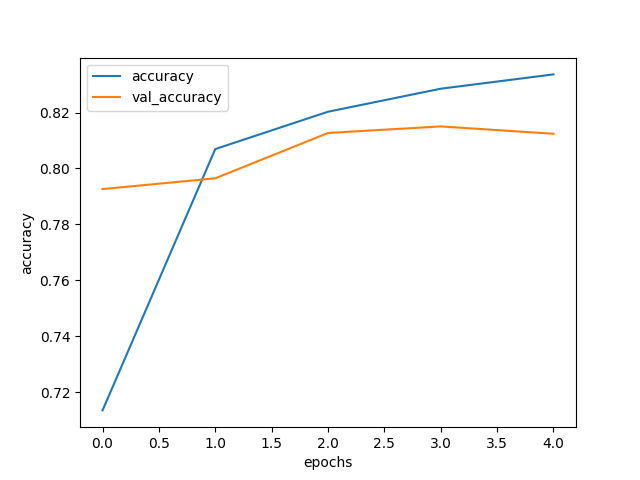
\includegraphics[scale=1]{Accuracy_Exp9}
	\label{fig:AccExp9}
	\captionsetup{type=figure}
	\setcounter{figure}{1}
	\caption{Accuracy values of the finished project}
\end{figure}


\section{Experiments}
Experiment 1: Base Experiment\\
Experiment 2: More Datasets With Reduced Data Scope\\
Experiment 3: Augmented LSTM Units\\
Experiment 4: Augmented Datasets Without Reduced Data
Scope\\
Experiment 5: Extra Sadness Dataset\\
Experiment 6: Reduced Classification Scope\\
Experiment 7: Reduced Epochs\\
Experiment 8: Added Stop Words\\
Experiment 9: Extra Stop Words and Reduced\\ Classification Scope\\ \\
\begin{table}[!h]
	\captionsetup{type=table}
	\setcounter{table}{1}
	\caption{Experiment results}
	\vspace{0.5cm}
	\centering
	\begin{tabular}[t]{|l|l|l|l|l|}
	\hline
	\multicolumn{1}{|c|}{} & \multicolumn{2}{c|}{Training} & \multicolumn{2}{c|}{Cross-Validation}
	\\ \hline
	\ & Loss & Accuracy & Loss & Accuracy
	\\ \hline
	\hyperref[exp1]{Experiment 1} & 0.6916 & 0.7130 & \textbf{0.8709} & 0.6234
	\\ \hline
	\hyperref[exp2]{Experiment 2} & 0.5956 & 0.7576 & 0.7649 & 0.6821
	\\ \hline
	\hyperref[exp3]{Experiment 3} & 0.5829 & 0.7564 & 0.7373 & 0.6780
	\\ \hline
	\hyperref[exp4]{Experiment 4} & 0.5455 & 0.7741 & 0.6704 & 0.7110
	\\ \hline
	\hyperref[exp5]{Experiment 5} & 0.5442 & 0.6620 & 0.6620 & 0.7162
	\\ \hline
	\hyperref[exp6]{Experiment 6} & 0.6222 & 0.6550 & 0.7186 & 0.5357
	\\ \hline
	\hyperref[exp7]{Experiment 7} & 0.6041 & 0.7451 & 0.6555 & 0.7097
	\\ \hline
	\hyperref[exp8]{Experiment 8} & 0.6030 & 0.7421 & 0.6579 & 0.7156
	\\ \hline
	\hyperref[exp9]{Experiment 9} & 0.3624 & 0.8337 & 0.3871 & \textbf{0.8124}
	\\ \hline
	\end{tabular}
\end{table}

\section{Conclusions}

These results determine that the proposed hypothesis is partially true: given enough data, a Machine Learning algorithm can learn to classify feelings and react accordingly, effectively learning how to identify patterns to an extent. However, high quality and volume data is needed for this to be reliable. Something that was only partially obtained for this project.

Overall, we can determine that, with the use of more consistent data, a favorable result can be achieved with the model used in this project.

\bibliography{biblio}
\bibliographystyle{unsrtnat}

\end{multicols}

\end{document}